\documentclass{article}
\usepackage[UTF8]{ctex}
\usepackage{newtxtext}
\usepackage{geometry}
\usepackage[dvipsnames,svgnames]{xcolor}
\usepackage[strict]{changepage} % 提供一个 adjustwidth 环境
\usepackage{framed} % 实现方框效果
\usepackage{setspace}
\usepackage{tikz}
\usepackage{tcolorbox}
\usepackage{amsmath}
\usepackage{graphicx}
\usepackage{wrapfig}
\usepackage{float}

\geometry{a4paper,centering,scale=0.8}

\definecolor{blueshade}{rgb}{0.95,0.95,1} % 文%本框颜色
\definecolor{greenshade}{rgb}{0.90,0.99,0.91} % 绿色文本框,竖线颜色设为 Green
\definecolor{redshade}{rgb}{1.00,0.90,0.90}% 红色文本框,竖线颜色设为 LightCoral
\definecolor{brownshade}{rgb}{0.99,0.97,0.93} % 莫兰迪棕色,竖线颜色设为 BurlyWood
\definecolor{yellowshade}{rgb}{1,0.945,0.7255}%米黄色
\definecolor{DarkYellow}{rgb}{0.7843,0.61176,0.0549}

\newenvironment{formal}[2][greenshade]{%
\def\FrameCommand{%
\hspace{1pt}%
{\color{#2}\vrule width 2pt}%
{\color{#1}\vrule width 4pt}%
\colorbox{#1}%
}%
\MakeFramed{\advance\hsize-\width\FrameRestore}%
\noindent\hspace{-4.55pt}% disable indenting first paragraph
\begin{adjustwidth}{}{7pt}%
\vspace{2pt}\vspace{2pt}%
}
{
\vspace{2pt}\end{adjustwidth}\endMakeFramed%
}



\title{\Huge 概率论与数理统计笔记    \\\large made by  \LaTeX}
\author{NP\_123}




\begin{document} 
\maketitle
\clearpage
\section*{\center\Huge 概率论的基本概念}
\begin{large}
\begin{tcolorbox}
    [colback=Emerald!10,colframe=cyan!40!black,title=\textbf{公式}]
    \center{$\overline{A\cup B}=\bar{A} \cap \bar{B} \hspace*{1cm} \overline{A\cap B}=\bar{A}\cup\bar{B}$}
    \[P(A-B)=P(A)-P(AB)=P(A\bar{B})\]
    \[P(A_1+A_2+A_3)=P(A_1)+P(A_2)+P(A_3)-P(A_1A_2)-P(A_1A_3)-P(A_2A_3)+P(A_1A_2A_3)\]
    \[P(A\cup B)=P(A)+P(B)-P(AB)\]
    \[P(AB)=P(A)P(B)\Longleftrightarrow \mbox{A与B独立}\]
\begin{nonumber}
\begin{align}
    \text{全概率公式:}\hspace{2cm}
    &P(A)=\sum_{i=1}^{n}P(A|B_i)P(B_i)\\
    \text{贝叶斯公式:}\hspace{2cm}
    &P(B_i|A)=\frac{P(B_i)P(A|B_i)}{\sum_{j=1}^{n}P(B_j)P(A|B_j)}=\frac{P(B_i)P(A|B_i)}{P(A)}
\end{align}
\end{nonumber}
\end{tcolorbox}
\end{large}

\begin{tcolorbox}
    [colback=brownshade,colframe=Sepia,title=\textbf{概念}]
    两两独立 $\neq$ 相互独立\\
    超几何分布与是否计序无关\\
    抽签原理:与抽签的次序无关
\end{tcolorbox}
\subsection*{模型}

\begin{itemize}
    \item 会面问题
    \item 莆丰投针
    \item 不放回抽样与二项分布
    \item 放回抽样与超几何分布
    \item 匹配问题
\end{itemize}
\clearpage
 
\section*{\center\Huge 随机变量的概率分布}
\begin{tcolorbox}
    [colback=greenshade,colframe=Green!50!black,title=\textbf{基本概念}]
    \[P(a<\xi\leq b )=F(b)-F(a) \hspace*{1cm} P(a\leq\xi< b)=F(b-0)-F(a=0)\]
    定理:若$g(x)$处处可导,恒有$g'(x)>0\text{或}g'(x)<0$,则$Y=g(X)$是连续型随机变量,概率密度
    \[f_Y(y)=\begin{cases}
        f_X[h(y)]\hspace{1pt}|h'(y)|,&\alpha<y<\beta ,\\
        0,&\text{其他},
    \end{cases}\]
    普通情况/证明
    \[
        \begin{split}
             F_Y(y)&=P\{Y\leq y\}=P\{g(X)\leq y\}\\
             &=P\{X\leq h(y)\}=F_X[h(y)]
        \end{split}
    \]
\end{tcolorbox}
\subsection*{离散型随机变量}
\begin{itemize}
    \item 单点分布\hspace*{0.5cm}$\xi \sim (x-c)$
    \[F(x)=\begin{cases}
            0& \text{, } x<c \\
            1& \text{, } x\geq c
           \end{cases}\]
    $E\xi =c \hspace*{1cm} D\xi =0$
    \item (0-1)分布\\
    \[P\{X=k\}=p^k(1-p)^{1-k}\hspace*{0.5cm}k=0,1\]
    $E\xi =p \hspace*{1cm} D\xi =p(1-p)$
    \item 二项分布\hspace*{0.5cm}$\xi\sim B (n,p)$
    \[P\{X=k\}=\binom{n}{k} p^k(1-p)^{1-k}\hspace*{0.5cm}k=0,1,2\cdots n\]
    \begin{figure}[H]
        \begin{center}
            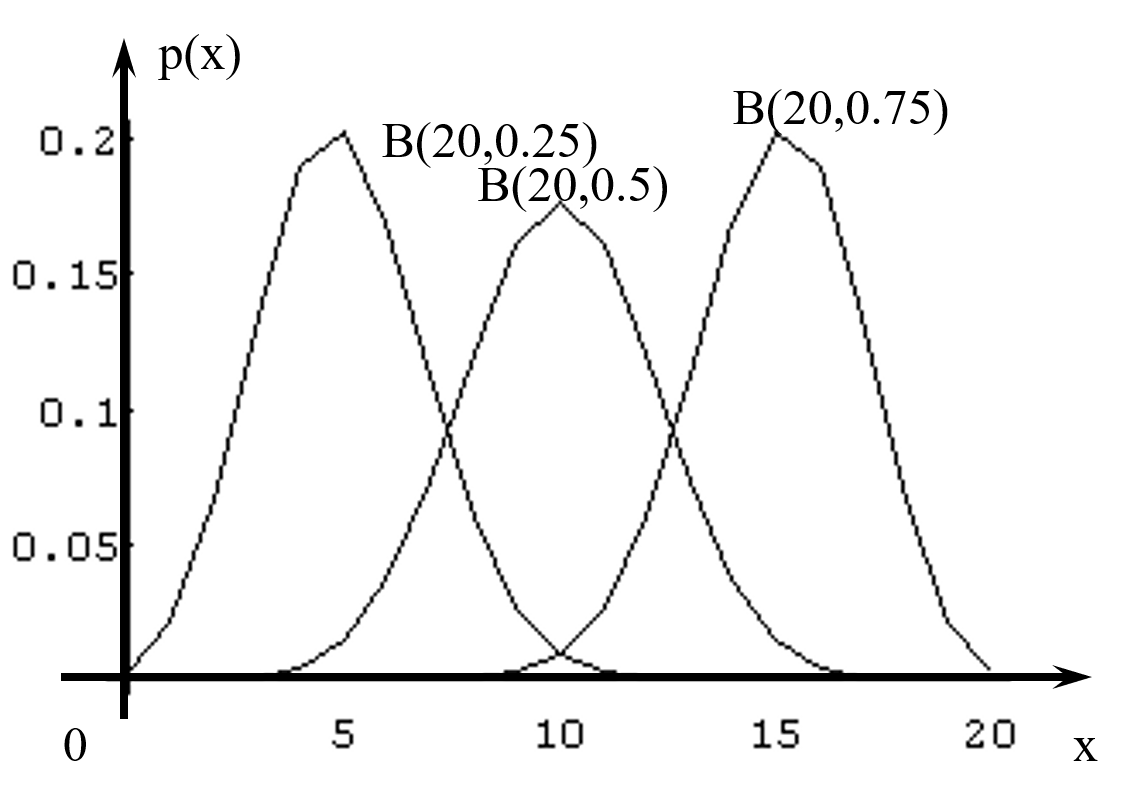
\includegraphics[width=0.3\textwidth]{Bernoulli}
            \caption{二项分布的概率密度函数}
        \end{center}
    \end{figure}
    $E\xi =np \hspace*{1cm} D\xi =np(1-p)$
    \item 泊松分布\hspace*{0.5cm}$\xi\sim P (\lambda)$
    \[P\{X=k\}= \frac{\lambda ^k}{k!}e^{-\lambda} \hspace*{0.5cm}k=0,1,2\cdots \]
    \begin{figure}[H]
        \begin{center}
            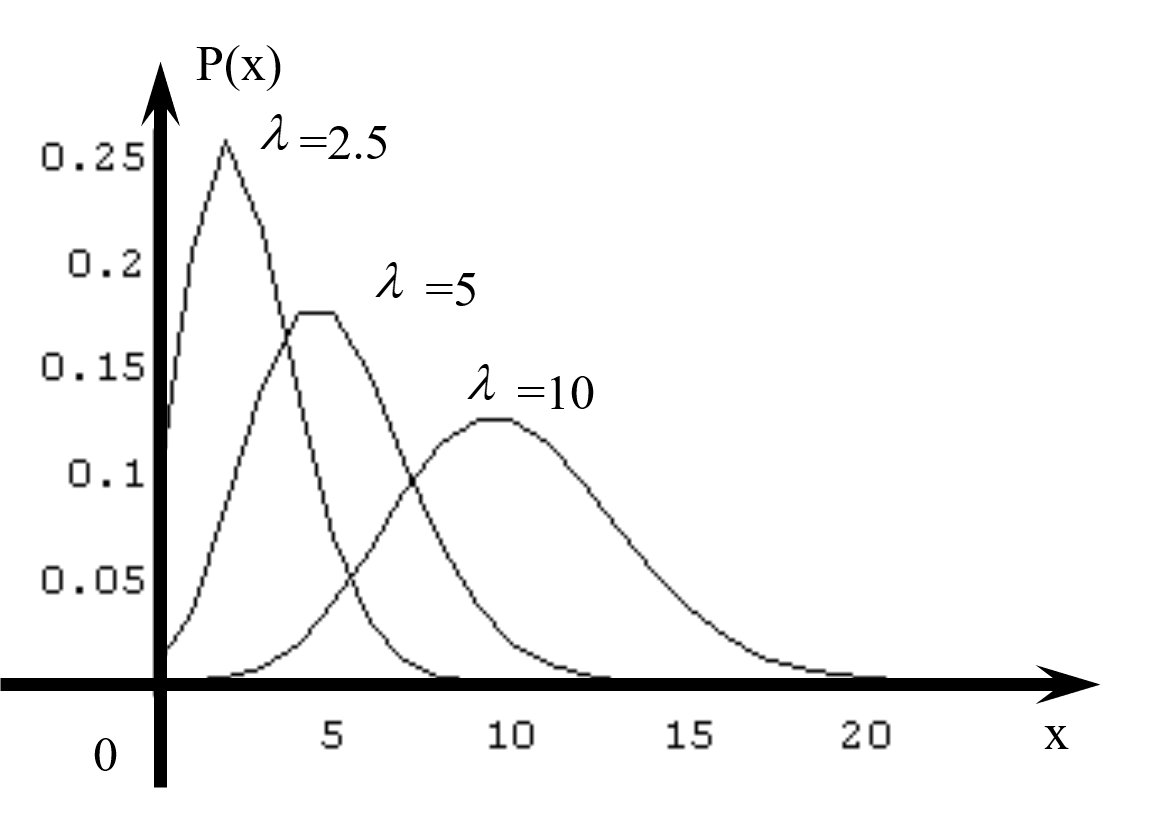
\includegraphics[width=0.3\textwidth]{Poisson.png}
            \caption{泊松分布的概率密度函数}
        \end{center}
    \end{figure}
    {\color{red}\textbf{注意:泊松分布是非对称的, 越大,非对称性越不明显。}}\\
    $E\xi =\lambda \hspace*{1cm} D\xi =\lambda$
    \item 超几何分布\hspace*{0.5cm}$\xi\sim H(n,M,N)$
    \[P\{X=k\}= \frac{C_M^kC_{N-M}^{n-k}}{C_N^n} \hspace*{0.5cm}k=0,1,2\cdots r=min(n,M)\]
    \item 几何分布\hspace*{0.5cm}$\xi\sim Ge(p)$\hspace*{1cm}首次成功发生在第k次
    \[P\{X=k\}= {(1-p)}^{k-1}p \hspace*{0.5cm}k=1,2,3\cdots \]
    p:A发生的概率\hspace*{1cm}$\xi$:A首次发生时的试验次数\\
    $E\xi =\frac{1}{p} \hspace*{1cm} D\xi =\frac{q}{p^2}$
\end{itemize}
\subsection*{连续型随机变量}
\begin{itemize}
    \item 均匀分布\hspace*{0.5cm}$\xi\sim U(a,b)$
    \begin{flalign*}
         p(x)=\begin{cases}
            \frac{1}{b-a} \text{, }& x\in (a,b) \\
            0 &\text{其他}
           \end{cases}\hspace*{1cm}
          F(x)=\begin{cases}
                0  \text{,}& x\leq a\\
                \frac{x-a}{b-a} \text{,}&a<x\leq b\\
                1 \text{,}&x>b
           \end{cases}
    \end{flalign*}
    $E\xi =\frac{a+b}{2} \hspace*{1cm} D\xi =\frac{{(b-a)}^2}{12}$
    \item 指数分布\hspace*{0.5cm}$\xi\sim E(\lambda)$\hspace*{1cm}寿命、某种服务的等待时间
    \begin{flalign*}
        p(x)=\begin{cases}
           \lambda e^{-\lambda x} \text{, }& x>0 \\
           0 \text{, }&x\leq 0
          \end{cases}\hspace*{1cm}
         F(x)=\begin{cases}
               1-e^{-\lambda x} \text{,}&a<x\leq 0\\
               0 \text{,}&x<0
          \end{cases}
   \end{flalign*}
   \begin{figure}[H]
    \begin{center}
        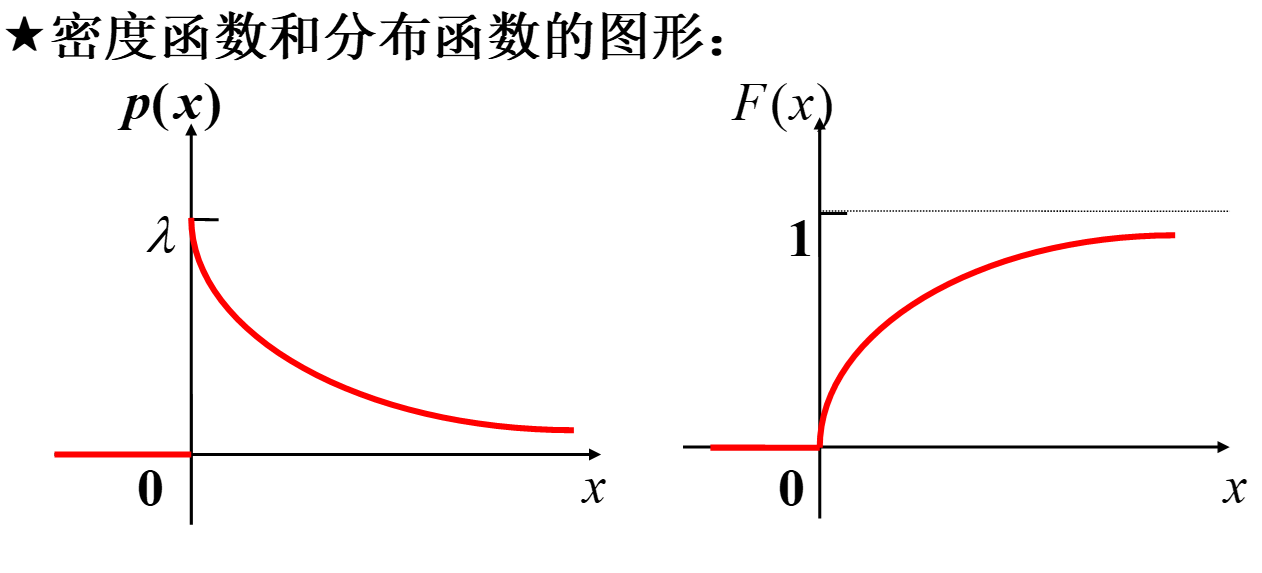
\includegraphics[width=0.6\textwidth]{Expon.png}
        \caption{指数分布}
    \end{center}
\end{figure}
$E\xi =\frac{1}{\lambda} \hspace*{1cm} D\xi =\frac{1}{\lambda ^2}$\\
{\color{red}$\star$ 模型:Poisson分布与指数分布的关系(电话,飞机)\hspace{1cm}无记忆性}
    \item 正态分布\hspace*{0.5cm}$\xi\sim N(\mu,\sigma )$\hspace*{1cm}$\star$3$\mu$原则
    \[p(x)= \frac{1}{\sqrt{2\pi}\sigma}e^{-\frac{{(x-\mu)}^2}{2\sigma^2}} \]
    {\color{red}\[\star \hspace{5pt}E(|X|)=\sqrt{\frac{2}{\pi}}\hspace{3cm}f_X(X^2)=\frac{1}{\sqrt{2\pi y}}e^{-\frac{y}{2}} \sim \chi ^2(1)\]}
\end{itemize}
\clearpage


\section*{\center\Huge 多元随机变量及其分布}

\noindent 二元正态分布:\hspace*{0.5cm}$\sim N(\mu_1,\mu_2,\sigma_1^2,\sigma_2^2,\rho)$
    \begin{enumerate}
        \item 联合正态$\Longrightarrow$边际正态
        \item 相同的边际正态,联合不一定正态
        \item 相同的边际正态,联合即使是正态,也可能不一样
    \end{enumerate}
    联合分布是均匀分布,但边缘分布都不是均匀分布。\\
    二项分布具有可加性:$\zeta =\xi +\eta \sim B(n_1+n_2,p)$\\
    泊松分布具有可加性:$\zeta =\xi +\eta \sim P(\lambda_1+\lambda_2)$\\
    正态分布具有可加性:$\zeta =\xi +\eta \sim N(\mu_1+\mu_2,\sigma_1^2+\sigma_2^2)$\\
    $\star$卷积公式:$p_\zeta(z)=\int_{-\infty}^{+\infty}p_\xi(x)p_\eta(y)|_{y=(z-x)}dx$\\
    一般的如果$Y =a\xi +b\eta $则
    \[p_{\zeta}(z)=\frac{1}{|b|}\int_{-\infty}^{+\infty}p_{\xi \eta}(x,y)|_{y=\frac{z-ax}{b}}dx\]
    商分布定理($Z=\frac{Y}{X}$、$Z=XY$):
    \[f_{Y/X}(z)=\int_{-\infty}^{+\infty}|x|\hspace{2pt}f(x,xz)dx\]
    \[f_{XY}(z)=\int_{-\infty}^{+\infty}\frac{1}{|x|}\hspace{2pt}f(x,\frac{z}{x})dx\]
    极值分布定理:
    \[F_{max}(z)={[F(z)]}^n\]
    \[F_{min}(z)=1-{[1-F(z)]}^n\]

$\star \Gamma$函数:
\[\Gamma(\alpha)=\int_{0}^{+\infty}x^{\alpha-1}e^{-x}dx\begin{matrix},&\alpha>0\\\end{matrix}\]
\begin{enumerate}
    \item $\Gamma(\alpha+1)=\alpha\Gamma(\alpha)$
    \item $\Gamma(n+1)=n!$
    \item $\Gamma(\frac{1}{2})=\sqrt\pi$
\end{enumerate}
\clearpage

\section*{\center\Huge 随机变量的数字特征}
\begin{nonumber}
\begin{align}
    \text{期望的函数嵌套:} \hspace{2cm}
        &E(Y)=E[g(X)]=\int_{-\infty}^{\infty} g(x)f(x)  \,dx  \\
    \text{切比雪夫不等式:}\hspace{2cm}
        &P\{|X- \mu | \geq \varepsilon\}\leq \frac{\sigma ^2}{\varepsilon ^2} \hspace{1cm}
        P\{|X-\mu|<\varepsilon\}\geq 1-\frac{\sigma ^2}{\varepsilon ^2}  \\
    \text{相关系数:}\hspace{2cm}
        &\rho_{XY} =\frac{\text{Cov}(X,Y)}{\sqrt{D(X)}\sqrt{D(Y)}}\\
    \text{协方差:}\hspace{2cm}
        &\text{Cov}(\xi,\eta)=E(\xi\eta)-(E\xi)\cdot(E\eta)\hspace{0.5cm}\text{Cov}(aX,bY)=ab\text{Cov}(X,Y)\\
        &\text{Cov}(X_1+X_2,Y)=\text{Cov}(X_1,Y)+\text{Cov}(X_2,Y)\\
        \hline
    \text{期望与方差基本公式:}\hspace{2cm}
        &E(CX)=CE(X)\hspace{1cm}E(X+Y)=E(X)+E(Y)\\
        &D(CX)=C^2D(X)\hspace{2cm}D(X+C)=D(X)\\
        &D(X)=E(X^2)-{[E(X)]}^2
    \end{align}
\end{nonumber}
\begin{itemize}
    \item 若独立则:\\
    $E(XY)=E(X)E(Y)$\\
    $D(X+Y)=D(X)+D(Y)$
    \item 非不独立则:\\
    $D(X+Y)=D(X)+D(Y)+2\hspace*{1pt}\text{Cov}(X,Y)$
\end{itemize}
{\color{red}$\star \xi $与$\eta$独立是 $\xi $与$\eta$不相关的充分不必要条件}

$\star$下车问题:20位旅客,十个车站可以下车,每个人每站下车的概率均等,设
\[X_i=\begin{cases}
    0,\text{在第i站没人下车}\\
    1,\text{在第i站有人下车}
\end{cases}\]
所以$X=X_1+X_2+\cdots +X_{10}$
\[E(X_i)=1-{(\frac{9}{10})}^{20}\]
\[E(X)=10[1-{(\frac{9}{10})}^{20}]=8.784\]


\section*{\center\Huge 数理统计}
\begin{tcolorbox}
    [colback=greenshade,colframe=Green!50!black,title=\textbf{基本概念}]
\begin{align}
    \text{卡方分布}\chi ^2 \sim \chi ^2(n)\hspace{2cm} 
    &\chi ^2=X_1^2+X_2^2+\cdots +X_n^2\\
    &E(X)=n \hspace*{2cm} D(X)=2n\\
    \text{t分布} t\sim t(n) \hspace{2cm}
    &t=\frac{X}{\sqrt{Y/n}}\\
    \text{F分布} F\sim F(n_1,n_2)\hspace{2cm}
    &F=\frac{U/n_1}{V/n_2}
\end{align}
定理:
\begin{enumerate}
    \item $\overline{X} \sim N(\mu ,\sigma^2/n)$
    \item $\frac{(n-1)S^2}{\sigma ^2}\sim \chi ^2(n-2)$
    \item $\overline{X}$与$S^2$相互独立
\end{enumerate}
区间估计评选标准:
\begin{enumerate}
    \item 无偏性
    \[E(\hat{\theta})=\theta \]
    \item 有效性
    \[D(\hat{\theta _1})\leq D(\hat{\theta _2})\]
    \item 相和性
    \[ \lim_{n\to \infty}P\{|\hat{\theta}-\theta\|< \varepsilon = 1 \}  \]
\end{enumerate}
枢轴量分布:
\begin{itemize}
    \item $\sigma^2$已知
    \[Z=\frac{\overline{X}-\mu}{\sigma /\sqrt{n}} \sim N(0,1)\qquad\text{置信区间:}(\overline{X} \pm \frac{\sigma}{\sqrt{n}}z_{\alpha/2})\]
    \item $\sigma^2$未知
    \[t=\frac{\overline{X}-\mu}{S /\sqrt{n}} \sim t(n-1)\qquad\text{置信区间:}(\overline{X} \pm \frac{S}{\sqrt{n}}t_{\alpha/2}(n-1))\]
\end{itemize}
\begin{center}
\begin{tabular}{c|c|c}
    \hline
    \multicolumn{3}{c}{假设检验中的两类错误}\\ \hline
    真实情况&\multicolumn{2}{c}{所作决策} \\  \cline{2-3}
    (未知)&接受$H_0$&拒绝$H_0$ \\ \hline
    $H_0$为真&正确&犯第I类错误\\ \hline
    $H_0$不真&犯第II类错误&正确\\ \hline
\end{tabular}
\end{center}
\end{tcolorbox}
\clearpage





\end{document}